\documentclass{article}

\usepackage{graphicx}
\usepackage{placeins}
\usepackage[subfigure]{ccaption}

\pagestyle{headings}

% italic captions with bold 'figure x'/'table y' texts
\captiontitlefont{\itshape}
\captionnamefont{\bf}


%
% Becuase figures are in pdf format, use
% ``pdflatex dm9ka_controller_doc.tex''
% to compile the sources
%

% *** START OF DOCUMENT ***
\begin{document}

\thispagestyle{empty} %no page numbering
\vspace*{4cm}
\centerline{\LARGE \textsc{DM9kA controller}}
\centerline{\rule{10cm}{1mm}}
\vspace{8cm}
\begin{flushright}
Written by: Jussi Nieminen\\
22.10.2009\\
Tampere University of Technology
\end{flushright}

\newpage

\thispagestyle{empty}
\tableofcontents

\newpage


\pagenumbering{arabic}


\section{INTRODUCTION}
DM9000A is an ethernet controller chip from Davicom. It is used e.g.
in Altera's DE2 FPGA board. \emph{DM9kA controller} is a VHDL based
hardware block, that is used to control the DM9000A. The source code
has a little over 2000 lines and the current version takes a little
over 900 logic cells in a Cyclone II with Quartus 9.0. Due to the
required operating frequency of the DM9000A, this controller block
also runs with 25~MHz clock signal.

\subsection{Interface}

The DM9000A is using a general processor interface with either 8-bit
or 16-bit data bus.  The DM9kA controller is made purely for the
16-bit version, the 8-bit version is not supported. Interface with the
DM9000A chip and the upper level (e.g. IP layer) is shown in
table~\ref{tab:interface}.

\begin{table}[htb]
  \begin{tabular}{|l|l|l|}
    \hline
    \textit{Signal} & \textit{Width} & \textit{Description} \\
    \hline
    eth\_clk\_out & 1 & 25 MHz clock signal to the DM9000A device. \\
    eth\_reset\_out & 1 & Reset signal. \\
    eth\_chip\_sel\_out & 1 & Chip select, active low. \\
    eth\_cmd\_out & 1 & Command signal, low for register address, high for data. \\
    eth\_write\_out & 1 & Write signal, active low. \\
    eth\_read\_out & 1 & Read signal, active low. \\
    eth\_data\_inout & 16 & Bidirectional data bus using tri-state buffers. \\
    eth\_interrupt\_in & 1 & Interrupt signal from the DM9000A chip. \\
    \hline
    new\_tx\_in & 1 & Goes high when upper level has a new transfer to send. \\
    tx\_len\_in & 11 & Length of the frame to be transferred. \\
    tx\_frame\_type\_in & 16 & Ethernet frame type. \\
    target\_MAC\_in & 48 & MAC address where to send. \\
    tx\_data\_in & 16 & Data to be transferred. \\
    tx\_data\_valid\_in & 1 & High when there is valid data waiting for reading. \\
    tx\_re\_out & 1 & Read enable signal to the upper level application. \\
    new\_rx\_out & 1 & Indicates that there is a new frame to be received. \\
    rx\_len\_out & 11 & Length of the received frame. \\
    rx\_frame\_type\_out & 16 & Ethernet frame type. \\
    rx\_erroneous\_out & 1 & High if frame is invalid (e.g. CRC checksum mismatch). \\
    rx\_data\_out & 16 & Received data. \\
    rx\_data\_valid\_out & 1 & High when received data is valid for reading. \\
    rx\_re\_in & 1 & Read signal from the upper level. \\
    \hline
    ready\_out & 1 & High when ethernet link is up and ready. \\
    fatal\_error\_out & 1 & Indicates serious malfunction in the DM9000A. \\
    \hline
  \end{tabular}
  \caption{DM9kA controller interface.}
  \label{tab:interface}
\end{table}


\vspace{1pc}
\noindent
\parbox{\textwidth}{
  \underline{\emph{IMPORTANT NOTICE:}}

  The 16-bit data busses consist of two bytes instead of a single 16-bit
  data word. Endianess of the data bus differs from an ethernet frame,
  so if you for example want to have a sequence 0xABCD in the ethernet
  frame, you need to write it as 0xCDAB to the data bus.
}


\subsection{Using the DM9000A}

The DM9000A is configured by first writing in a register address and
then writing data to that register. The command signal (eth\_cmd\_out)
decides whether the value being written is an address or actual data.
Transfer data is written in by selecting the register address of
transfer data buffer and then writing to it. Data is received by first
writing the register address of the received data buffer and then
reading from it.


% don't let figures/tables get any further
\FloatBarrier
\newpage

\section{MODULES}

DM9kA controller is formed of five different modules as shown in
figure~\ref{fig:modules}.  Comm (meaning communication) module talks
with the DM9000A chip and relays to it configuration data from the
other modules. These other modules (except Init) compete from Comm's
attention by raising up comm request signals. They have fixed
priorities that are located in the lower right corners of the boxes in
the figure. Once a module gets the turn (comm grant signal goes up) it
cannot be taken away from the module before it lowers its request
signal. Init module has it's turn when the controller is released from
reset and the module is no longer needed after the chip has been
initialized and the ethernet link is up.

\begin{figure}[htb]
  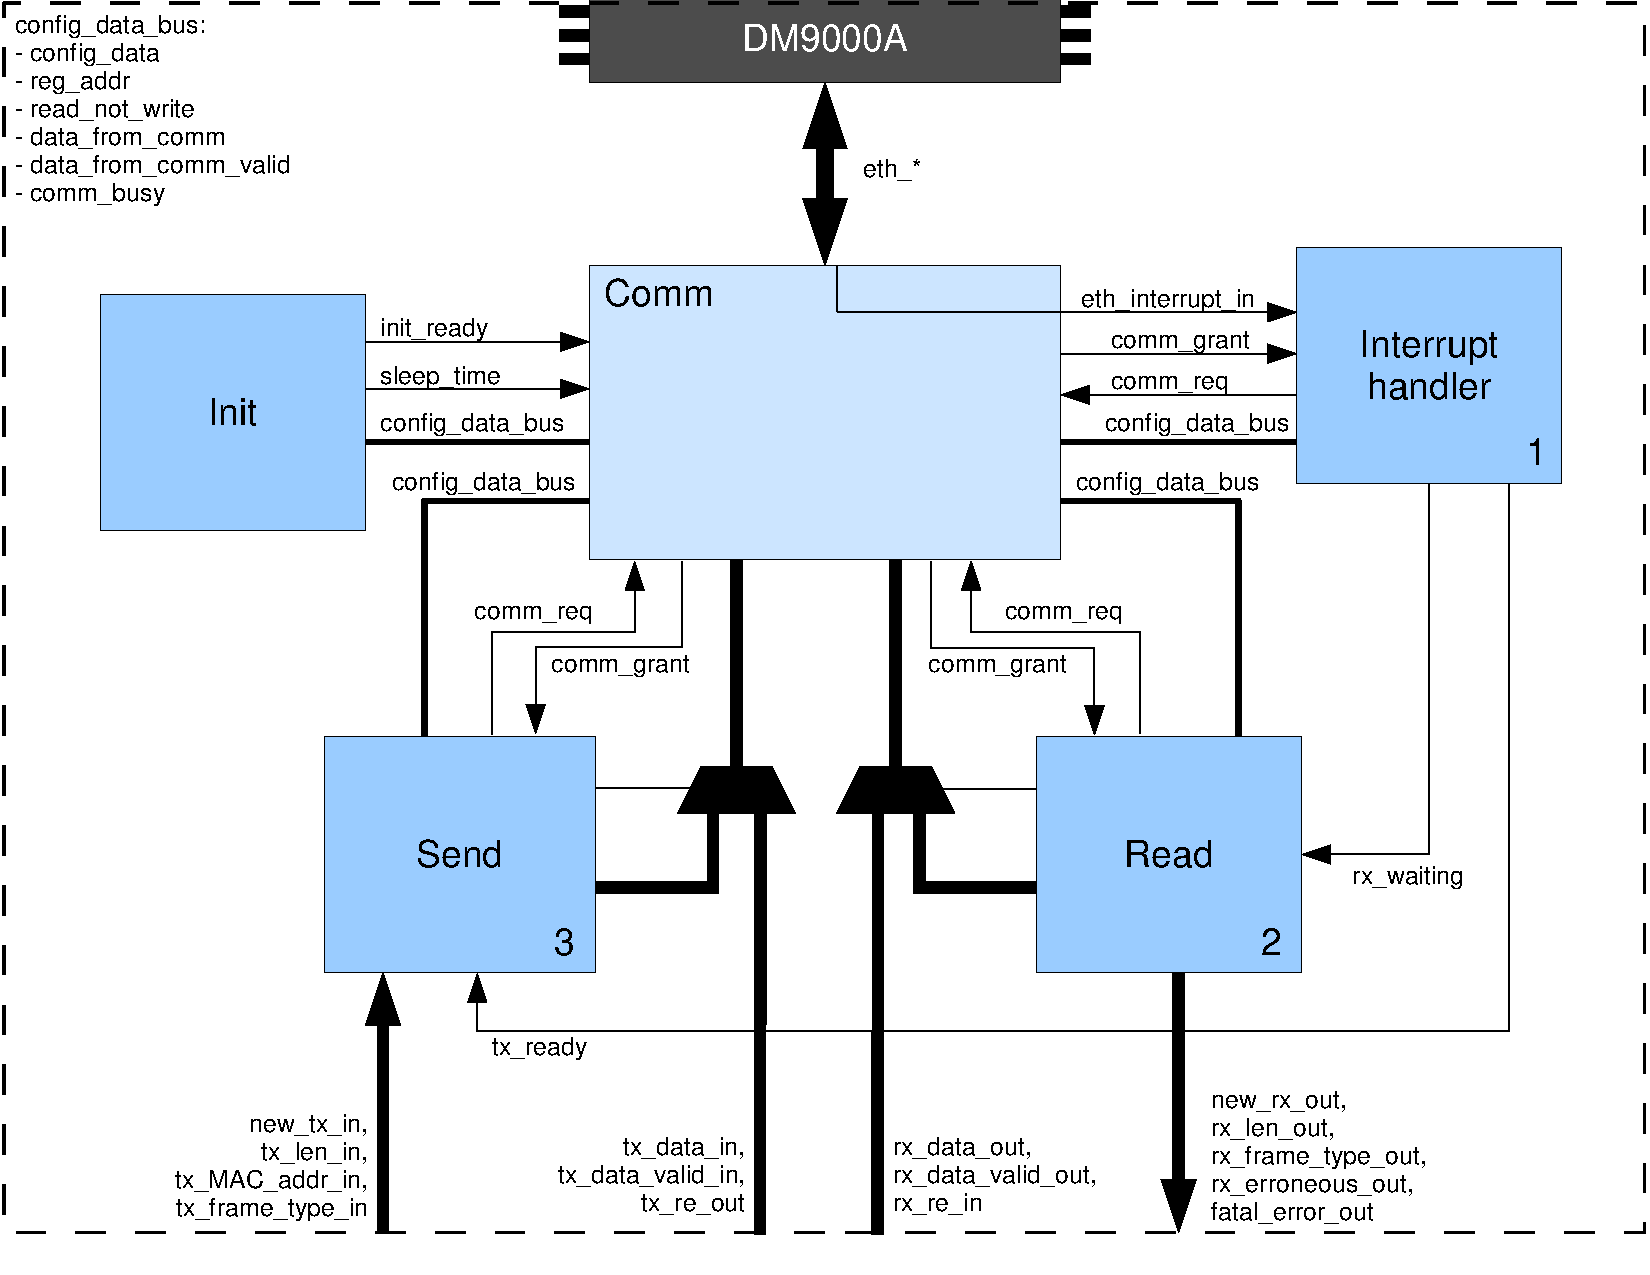
\includegraphics[scale=.5]{modules}
  \caption{DM9kA controller modules.}
  \label{fig:modules}
\end{figure}

\subsection{Comm module}

As told before, Comm module handles communication with the DM9000A
chip. It's also responsible for the arbitration between Interrupt
handler, Read module and Send module. Comm module gets the
configuration data and returns read values via configuration data
buses (see table~\ref{tab:confDataBus}). Other modules don't have to
worry about timing or other details concerning communication with the
chip, so it should be relatively easy to convert this controller to
use another ethernet controller than DM9000A. (Or then it's even
harder, don't know, but at least it is supposed to be easy..)

Comm module has three main states, config state where it writes or
reads configuration data and write/read data states for relaying
transfered data. Those latter states are entered when the register
addresses of TX or RX buffers are written to the device in the config
state. Data is read/written straight from/to the upper level to
eliminate unnecessary latency.

\begin{table}[hb]
  \begin{tabular}{|l|l|l|}
    \hline
    \textit{Signal} & \textit{Width} & \textit{Description} \\
    \hline
    config\_data & 8 & Data to be written to the specific register. \\
    reg\_addr & 8 & Address of the configuration register. \\
    read\_not\_write & 1 & If high, read the value of the register instead of writing. \\
    data\_from\_comm & 8 & If read\_not\_write is high, the value of the register. \\
    data\_from\_comm\_valid & 1 & Register value is valid to be read. \\
    comm\_busy & 1 & High when the Comm module is working. \\
    \hline
  \end{tabular}
  \caption{Signals of the configuration data bus.}
  \label{tab:confDataBus}
\end{table}


\subsection{Init module}

Init module is responsible for initializing the DM9000A chip. It
contains the initialization values and tells the Comm module to write
them to the chip. The values are stored in an array that the module
goes trought during initialization. Table~\ref{tab:initValues} shows
the parameters contained by a single array element. The initialization
process is thus easily modified by editing, removing or adding elements
to the table. One must just remember to update the array size constant
too, if the number of elements in the array changes.

\begin{table}[hbt]
  \begin{tabular}{|l|l|}
    \hline
    \textit{Parameter} & \textit{Description}\\
    \hline
    Address & Address of the register that is accessed.\\
    Value & Value that is written to the register.\\
    Write & If '1', write the value to the register, otherwise read\\
    & the register's contents and ignore the Value field.\\
    Sleeping time & Some operations require some waiting, so the Comm\\
    & module stays idle as many cycles as the Sleeping time shows.\\
    \hline
  \end{tabular}
  \caption{Contents of a single initialization array element.}
  \label{tab:initValues}
\end{table}

After initialization the module waits and polls the link status bit of
the DM9000A chip to know when the link is up and the chip is ready for
transmissions. After the link status is up, the module waits few more
seconds for the link on the other side to be ready as well and then
notifies the Comm module about initialization being complete.  The
Init module has the Comm modules complete attention as long as the
ready bit has not been risen. When done, Init module becomes idle
until next reset.




\subsection{Interrupt handler module}

Interrupt handler does exactly what the name suggests. It handles
interrups from the DM9000A. The \emph{eth\_interrupt\_in} signal is
connected straight to the handler, but it needs Comm module to know
why the interrupt has been risen.

Only two sorts of interrupts are handled. If there is a new received
transmission waiting, the Interrupt handler raises the
\emph{rx\_waiting} signal that goes to Read module.  The other handled
interrupt tells that an outgoing transfer has been completed. In that
case the handler raises the \emph{tx\_ready} signal.


\subsection{Read module} \label{sec:readModule}

Read module wakes up and starts requesting a turn when signal
\emph{rx\_waiting} is lifted up by Interrupt handler. Module's state
machine is shown in figure~\ref{fig:readStates}. Data comes from
the chip as shown in table~\ref{tab:rxdata}. The leading 0x01 byte
means that there is a new frame waiting. In theory the value of the
first byte should always be peeked first without reading it away from
the buffer. We know from the interrupt when there is a new received
frame but we still do a dummy peek to the buffer (see
section~\ref{sec:peekingFail} for details why).

After peeking (and a little delay) we start reading values for real.
The peeked byte is still there, and in state check\_first\_byte we
read it away from the buffer and check that it is correct. It has to
be 0x01 (standing for a new frame), because this state is not entered
without a received frame available interruption from the DM9000A chip.
If the byte is something else than 0x01, we stop doing anything and go
to the fatal\_error state.

Status byte contains the same information than DM9000A's RX status
register.  Bit 7 tells us that the incoming frame has a multicast
address (not so serious) but all the others stand for different
errors. So if other than bit number 7 is up, we raise up the
\emph{rx\_erroneous} signal. The frame still gets sent to the upper
level, which can decide what to do with it.

After the status check we get the frame length and strip away the
ethernet header (source and destination addresses and ethernet frame
type field) and start relaying the data to the upper level. The last
two bytes form a CRC checksum that has already been checked by the
DM9000A chip, so it's just stripped away from the data. Last thing to
do is to peek the next value in the buffer to check whether there is
another frame waiting (0x01) or not (0x00). Once again any other value
means that there is something seriously wrong.

If there is another frame, it might have arrived when we were reading
out the first one. This means that there must be an RX interrupt waiting
to be handled by the Interrupt handler. The interrupt must be cleared so
that the handler doesn't inform us about a frame that we have already
read out from the RX buffer.

\begin{figure}[hbt]
  \includegraphics[scale=.4]{Read_module_states}
  \caption{State machine of the Read module.}
  \label{fig:readStates}
\end{figure}

\begin{table}[hb]
  \begin{tabular}{|l|l|l|l|l|l|l|l|l|}
    \hline
    0x01 & status & length low & length high & data & \ldots & CRC 1 & CRC 2 & 0x00/0x01 \\
    \hline
  \end{tabular}
  \caption{Format of RX data in the RX data buffer. One cell equals one byte.}
  \label{tab:rxdata}
\end{table}


\subsection{Send module}

\begin{figure}[hbt]
  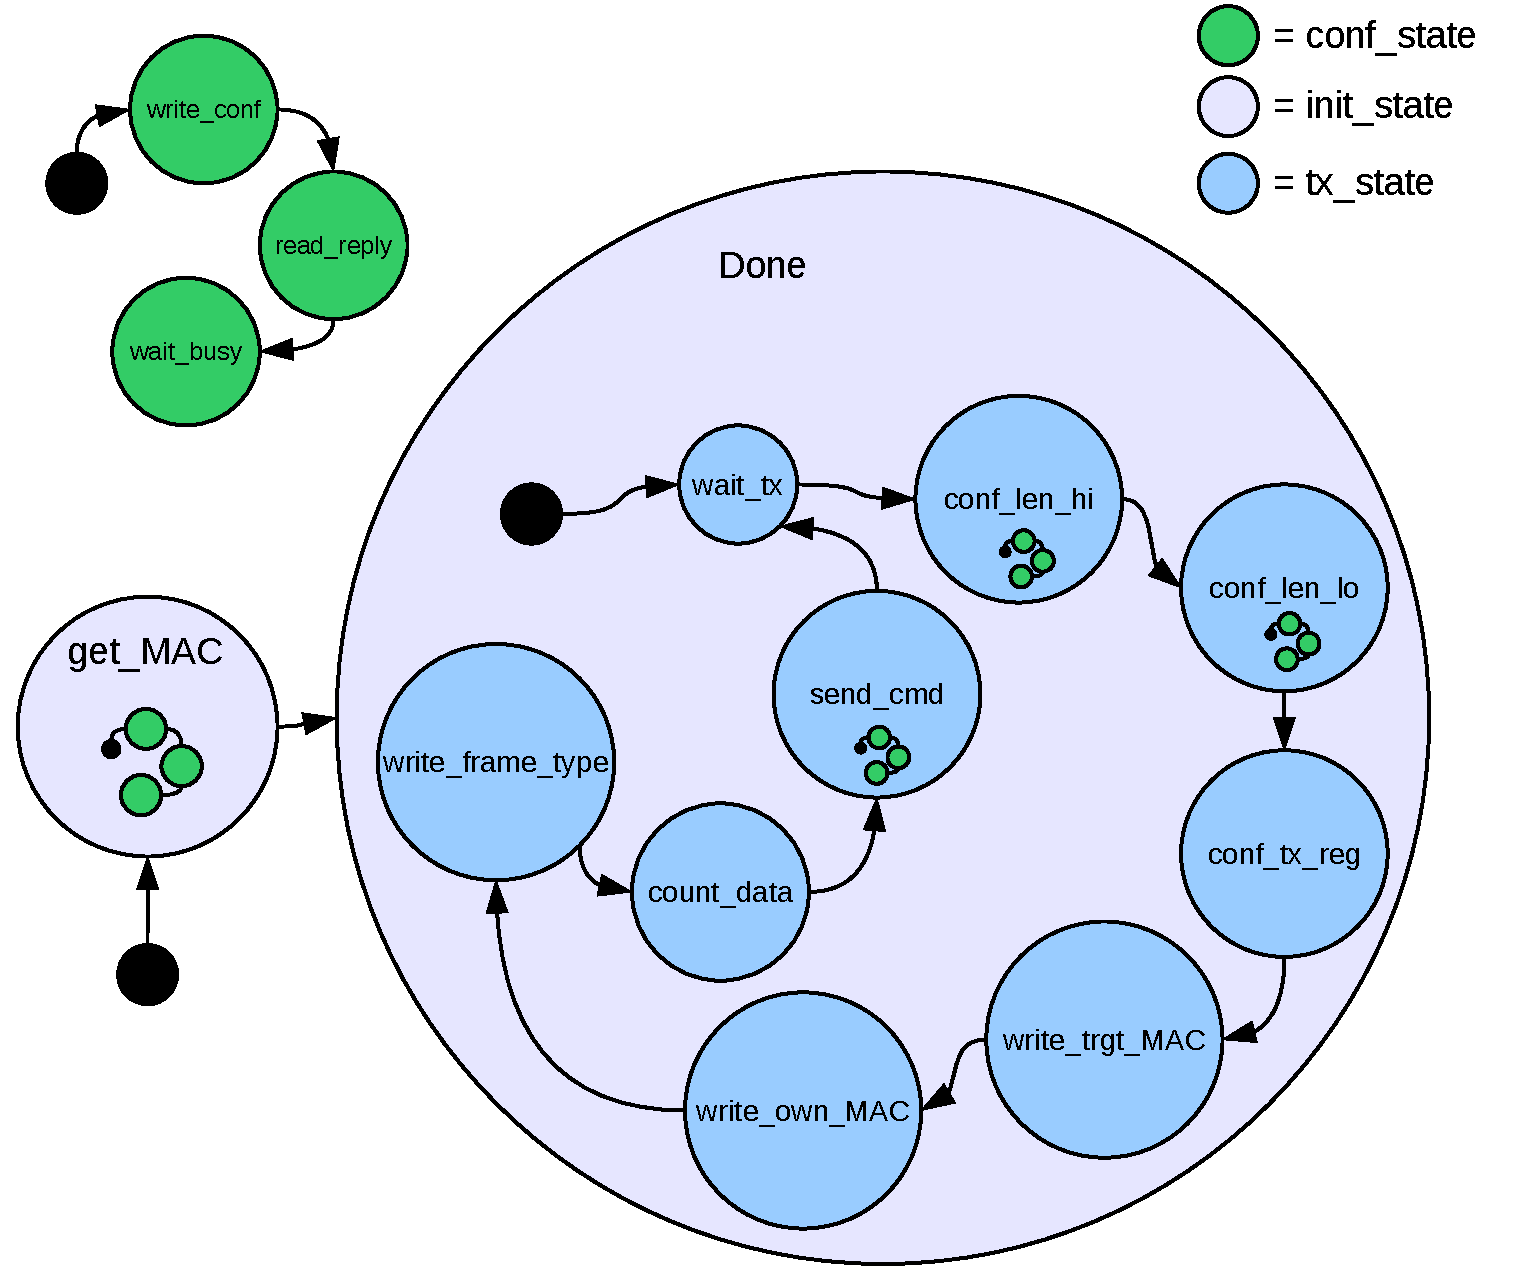
\includegraphics[scale=.5]{send_module_states}
  \caption{State machines of the Send module.}
  \label{fig:sendStates}
\end{figure}

Like the monstrous diagram in figure~\ref{fig:sendStates} tries to
explain, Send module consists of three different state machines.
Conf\_state is used every time the module has to configure or read
DM9000A's configuration registers. The init\_state state machine is
more or less a relic from earlier design phases and nowdays its only
function is to separate normal running state (named 'done') from the
state where we fetch our own MAC address from the DM9000A right after
reset.

The tx\_state is really the main state machine in the module. It stays
in the wait\_tx state until upper level application announces that it
wants to send something. Next job to do is to store transfer length to
the DM9000A's registers. After that we set the send buffer address to
the chip. This also tells the Comm module to start relaying data
straight to the buffer.

Send module is responsible of writing the ethernet header to the
frame.  The header consists of destination address (usually called
'target address' in the code), source address (that we fetched in the
get\_MAC state of init\_state state machine) and ethernet frame type,
that for example separates ARP packets from IP packets.

After writing the header the Send module starts to relay data from
upper level application to the Comm module. It keeps track of the
amount of data that has already been written and knows when to stop
relaying. After data has been written the Send module raises TX
Request bit of DM9000A's TX Control Register. This is not always
necessary because the chip can be configured to start transmitting
automatically after certain percentage of the data is written to the
buffer. There is a constant \emph{send\_cmd\_en\_c} in the code that
decides whether the send command is given or not.


\newpage
\section{RESTRICTIONS AND WEIRD STUFF}

\subsection{Intended use}

This controller is meant to be simple and small, so it's not possible
to use all of the features supported by DM9000A. Also the main
goal is to support predetermined communication between Altera's DE2
board and a single PC and for example status bits warning about
collisions are not monitored.  All in all, using this DM9kA controller
to connect DE2 to a network may work, but problems will arise once
something a bit unusual happens.


\subsection{Performance}

The DM9000A chip can read or write two bytes of data every second
clock cycle. With 25~MHz clock this means bandwidth of 25~MB/s or
200~Mbit/s. At the moment this controller block is reading received
data only once in three cycles, so rx bandwidth is really 16.7~MB/s or
133~Mbit/s. If higher rate is needed, Comm module's
\textit{read\_data} state has to be modified. Highest measured
bandwidth of the ethernet bus with the DM9000A chip using this block
was 97.4~Mbit/s.


\subsection{Initializing device}

The DM9000A is a bit curious device and its datasheets are not too
helpful. There are instructions in the DM9000A Application Notes about
initializing the chip, but at least I couldn't get the thing working
following them. Altera's example code that came with the DE2 revealed,
that some tricks have to be done (like turning on and off the PHY) in
order to get the chip up and running. After getting the chip to work,
I didn't give the initialization process too much attention, so there
might be some redundancy.

\subsection{Using the RX buffer} \label{sec:peekingFail}
% peeking rx buffer doesn't work

Reading from DM9000A's control register 0xF0 is supposed to return the
first value in the RX data buffer without incrementing the buffer's
pointer. So the value is just peeked without removing it from the
buffer. This is meant to be used when checking whether there is
something to be read in the buffer (see section~\ref{sec:readModule}).
But every time the RX buffer is used after some other operations, the
first peek to it returns something completely different than the first
value. The same invalid value is also returned, if we are using
register 0xF2 (that increments the buffer pointer) as the first read
operation.

DM9000A's data sheet doesn't really explain this, but it gives some
hints what to do and why. In an example C code there is a dummy read
using the 0xF0 register. The returned value isn't used in any way. The
description of the 0xF0 register in the data sheet also states that by
reading the register value \emph{''the DM9000A starts to pre-fetch the
  SRAM data to internal data buffers''}. They just forgot to mention,
that the first read operation apparently returns some old random value
from those internal data buffers and only after that you can start
reading the correct data.



\end{document}
